\section{Лекция 7.06.2018}

\subsection{Эллипс}

$\frac{x^2}{a^2} + \frac{y^2}{b^2} = 1, a \geqslant b > 0$

\bigskip
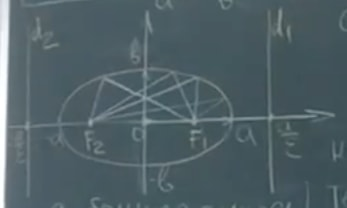
\includegraphics[width=10cm,height=15cm,keepaspectratio]{example3.jpg}

\bigskip
$a$ -- большая полуось, $b$ -- малая полуось

$c = \sqrt[]{a^2 - b^2}$

$0 \leqslant c < a$

Точки $F_1(c, 0), F_2(-c, 0)$ называются \textit{фокусами} эллипса.

\bigskip
\textbf{Теорема.} Точка $P$ лежит на эллипсе $\Leftrightarrow \rho(P, F_1) + \rho(P, F_2) = 2a$

\bigskip
$\epsilon = \frac{c}{a}, 0 \leqslant \epsilon \leqslant 1$ -- эксцентралитет эллипса

\bigskip
Прямые $d_1: x = \frac{a}{\epsilon}, d_2: x = -\frac{a}{\epsilon}$ называются \textit{директрисами} эллипса.

\bigskip
\textbf{Теорема.} Точка $P$ лежит на эллипсе $\Leftrightarrow \frac{\rho(P, F_i)}{\rho(d_i)} = \epsilon$

\bigskip
\textbf{\textit{Оптическое свойство эллипса:}} Лучи света, выпущенные из одного фокуса, после отражения от стенок собираются в другом фокусе.

\subsection{Гипербола}

$\frac{x^2}{a^2} - \frac{y^2}{b^2} = 1, a \geqslant b > 0$

\bigskip
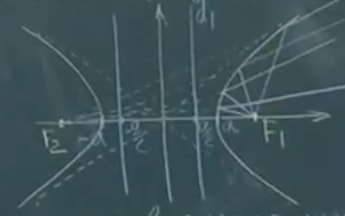
\includegraphics[width=10cm,height=15cm,keepaspectratio]{example4.jpg}

\bigskip
$a$ -- действительная полуось, $b$ -- мнимая полуось

\bigskip
$y = \frac{b}{a}x, y = - \frac{b}{a}x$ -- асимптоты

$c = \sqrt[]{a^2 + b^2}, c > a$

$F_1(c, 0), F_2(-c, 0)$ -- фокусы

\bigskip
\textbf{Теорема.} $P$ лежит на гиперболе $\Leftrightarrow |\rho(P, F_1) - \rho(P, F_2)| = 2a$

\bigskip
$\epsilon = \frac{c}{a}, \epsilon > 1$

\bigskip
Директрисы: $d_1: x = \frac{a}{\epsilon}, d_2: x = -\frac{a}{\epsilon}$

\bigskip
\textbf{Теорема.}  Точка $P$ лежит на гиперболе $\Leftrightarrow \frac{\rho(P, F_i)}{\rho(d_i)} = \epsilon$

\bigskip
\textbf{\textit{Оптическое свойство гиперболы:}} Лучи света, выпущенные из одного фокуса, после отражения от стенок идут так, как будто они были выпущены из другого фокуса.

\subsection{Парабола}

$y^2 = 2px, p>0$

\bigskip
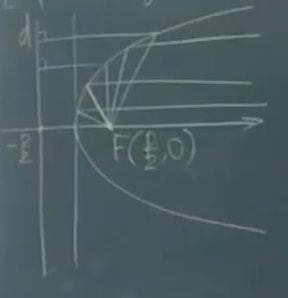
\includegraphics[width=10cm,height=15cm,keepaspectratio]{example5.jpg}

\bigskip
Фокус: $F(\frac{p}{2}, 0)$

Директриса: $d: x = \frac{p}{2}$

$\epsilon = 1$

\bigskip
\textbf{Теорема.} Точка $P$ лежит на гиперболе $\Leftrightarrow \rho(P, F) = \rho(P, d)$

\bigskip
\textbf{\textit{Оптическое свойство параболы:}} Лучи света, выпущенные из фокуса, после отражения от стенок идут параллеьно оси $Ox$.

\bigskip
Эллипс, гипербола и парабола называются кониками (или коническими сечениями)

\bigskip
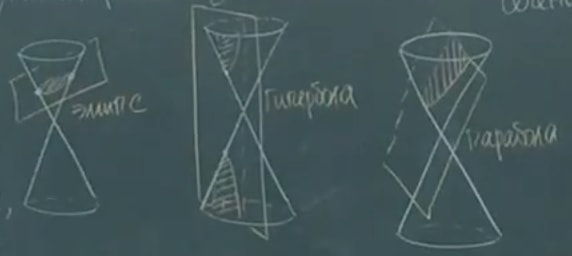
\includegraphics[width=10cm,height=15cm,keepaspectratio]{example6.jpg}

\subsection{Жорданова нормальная форма}

$V$ -- векторное пространство над полем $F$

$\varphi: V \rightarrow V$ -- линейный оператор

\bigskip
\textbf{\textbf{Критерий диагонализуемости:}}

$\varphi$ диагонализуем $\Leftrightarrow$

1) $\chi_{\varphi} (t) = (t - \lambda_1)^{k_1} \dots (t = \lambda_s)^{k_s}$

2) $\forall \ i: k_i = dim V_{\lambda_i} (\varphi)$

\bigskip
\textbf{Теорема (о Жордановой нормальной форме).} Пусть выполнено условие 1), т.е. $\chi_{\varphi} (t) = (t - \lambda_1)^{k_1} \dots (t - \lambda_s)^{k_s}$. Тогда $\exists$ базис $e$ в $V$, такой что \begin{equation*}A(\varphi, e) = \left(
\begin{array}{c|c|c|c|c}
  J^{m_1}_{\mu_1} & 0 & 0 & \dots & 0  \\
  \hline
  0 & J^{m_2}_{\mu_2} & 0 & \dots & 0  \\
  \hline
  0 & 0 & J^{m_3}_{\mu_3} & \dots & 0 \\
  \hline
  \vdots & \vdots & \vdots & \vdots & \vdots \\
  \hline
  0 & 0 & 0 & \dots & J^{m_p}_{\mu_p} \\
\end{array}
\right) (*)\end{equation*}

где $J^{m_i}_{\mu_i} = \begin{pmatrix} \mu_i & 1 & 0 & \dots & 0 \\ 0 & \mu_i & 1 & \dots & 0 \\ 0 & 0 & \mu_i & \dots & 0
\\ \vdots & \vdots & \vdots & \vdots & \vdots \\ 0 & 0 & 0 & \dots & \mu_i \end{pmatrix}$ -- Жорданова клетка порядка $m_i$ с собственным значением $\mu_i$

$\{\mu_1, \dots, \mu_p\} = Spec \varphi = \{\lambda_1, \dots, \lambda_p\}$

\bigskip
Более того, вид $(*)$ определен однозначно с точностью до перестановки клеток.

\bigskip
$\varphi \in L(V), \chi_{\varphi} (t) = (t - \lambda_1)^{k_1} \dots (t - \lambda_s)^{k_s}$

$\lambda \in Spec \varphi$

\bigskip
\textbf{Определение.} Вектор $v \in V$ называется \textit{корневым вектором линейного оператора} $\varphi$, отвечающим собственному значению $\lambda$, если $\exists \ m \geqslant 0$, такое что $(\varphi - \lambda \cdot Id)^m v = 0$.

При этом наименьшее такое $m$ называется \textit{высотой} корневого вектора $v$. Обозначение: $ht(v)$

\bigskip
$ht(v) = 0 \Leftrightarrow v = 0$

$ht(v) = 1 \Leftrightarrow (\varphi - \lambda \cdot Id) v = 0 \Leftrightarrow \varphi(v) = \lambda v \Leftrightarrow v$ -- собственный вектор с собственным значением $\lambda$

\bigskip
$V^{\lambda} (\varphi)$ -- множество всех корневых векторов, отвечающих собственному значению $\lambda$

\bigskip
\textbf{\textit{Упражнение.}} $V^{\lambda} (\varphi)$ -- подпространство в $V$

\bigskip
\textbf{Определение.} $V^{\lambda} (\varphi)$ называется \textit{корневым подпространством}, отвечающим собственному значению $\lambda$

\bigskip
\textbf{Замечание.} $V_{\lambda} (\varphi) \subseteq V^{\lambda} (\varphi)$

\bigskip
Пример.

$V = F[x]_{\leqslant n}, char F = 0$

$\varphi: f \rightarrow f'$

$\chi_{\varphi}(t) = t^{n+1}, Spec \varphi = \{0\}$

$V^0 (\varphi) = V$

$F \in V \Rightarrow deg(f) = k \Leftrightarrow ht(f) = k + 1$

\bigskip
\textbf{Факты.}

1) $V^{\lambda} (\varphi) \ \varphi$-инвариантно

2) $dim V^{\lambda} (\varphi) = $ алгебраической кратности собственного значения $\lambda$

3) Если $\lambda_1, \dots, \lambda_k \in Spec \varphi, \lambda_i \neq \lambda_j$ при $i \neq j$, то $V^{\lambda_1} (\varphi) \dots V^{\lambda_k} (\varphi)$ линейно независимы

\bigskip
\textbf{Следствие.} Если $\chi_{\varphi} (t) = (t - \lambda_1)^{k_1} \dots (t - \lambda_s)^{k_s}$, то $V = V^{\lambda_1} (\varphi) \oplus \dots \oplus V^{\lambda_s} (\varphi)$

\bigskip
Если $e_i$ -- базис в $V^{\lambda} (\varphi)$ и $e = e_1 \sqcup e_1 \sqcup \dots \sqcup e_s$, то \begin{equation*}A(\varphi, e) = \left(
\begin{array}{c|c|c|c|c}
  A_1 & 0 & 0 & \dots & 0  \\
  \hline
  0 & A_2 & 0 & \dots & 0  \\
  \hline
  0 & 0 & A_3 & \dots & 0 \\
  \hline
  \vdots & \vdots & \vdots & \vdots & \vdots \\
  \hline
  0 & 0 & 0 & \dots & A_s \\
\end{array}
\right)\end{equation*}

$A_i = A(\varphi|_{V^{\lambda_i} (\varphi)}, e_i)$

$\Rightarrow$ доказательство теоремы о ЖНФ сводится к случаю $V = V^{\lambda_i} (\varphi)$

Далее считаем, что $Spec \varphi = \{ \lambda\}, \chi_{\varphi} (t) = (t - \lambda)^n, n = dim V$

$V = V^{\lambda} (\varphi)$

Полагая $\psi = \varphi - \lambda \cdot Id$, получаем $\chi_{\psi} (t) = t^n, Spec \psi = \{0\}, V = V^0 (\psi)$

Далее считаем $Spec \varphi = \{0\}$

\bigskip
\textbf{Определение.} Линейный оператор называется \textit{нильпотентным}, если $\exists m \in \NN$, такой что $\varphi^m = 0$

\bigskip
Фиксируем наименьший $m$, такой что $\varphi^m = 0$. Имеем $0 = Ker \varphi^0 \subseteq \overbrace{Ker \varphi^1}^{собственное \ подпространство} \subseteq Ker \varphi^2 \subseteq \dots \subseteq Ker \varphi^m = V$

